\section{Limits from Muon Decays in \mueee Experiment}
In section \ref{sec:mu3e_experiment}, we saw how the production rate of $\mu^+$ at \mueee could be brought to the level of muon decays occurring at a rate $\order(10^9)~\mu^+/\textrm{s}$.
The signal for the \mueee experiment, $\mu^+ \rightarrow e^+ e^+ e^-$, contains no missing energy as there are no neutrinos in the final state.
The SM has many avenues to produce such a signal with missing energy through muon decay, and we will go through the relevant backgrounds for our sensitivity limits here.
Since the experiment consists of many muons stopped in a target, it can be expected that there will be many events that behave like a muon decay and have missing energy.
Our signal will overlap with the backgrounds present and \mueee, and will allow us to study the signal component of $\mu^+ \rightarrow e^+ \bar{\nu}_\mu \nu_e e^+ e^-$.

For this experiment, we have utilized \madgraph to do the final state integration, as our signal will have four particles in the final state and this is difficult to do by hand.
Furthermore, even though we will be looking at a four body decay, the scalar particle will be on-shell and decay later to an $e^+ e^-$ pair, and \madgraph will also take care of generating the events corresponding to this decay.
All of the diagrams that \madgraph generates are available in appendix \ref{app:muon_diagrams}.

\subsection{Backgrounds}
Here we will discuss the relevant backgrounds to the proposed signature and their implications/effects on our sensitivity limits.

A large irreducible background for the experiment is

\begin{equation}
    \mu^+ \rightarrow e^+ + \bar{\nu}_\mu + \nu_e + e^+ + e^-
\end{equation}

\noindent which comes with a branching ratio of $3.4 \times 10^{-5}$ \cite{Agashe:2014kda}. 
This is due to an internal conversion of muon to electron with a weak vertex, just like an ordinary muon decay (also known as a Michel decay.)
To remove this background process, momentum conservation can be applied provided that the energy resolution is small enough.
For \mueee, a total energy resolution of $\sigma_E < 1\textrm{MeV}$ is sufficient for sensitivity of branching ratios down to $10^{-15}$ \cite{Blondel:2013ia}.
One such diagram for this process is shown in Fig.\ \ref{fig:mu_eeenunu_SM}.

\begin{figure}[h]
    \centering
    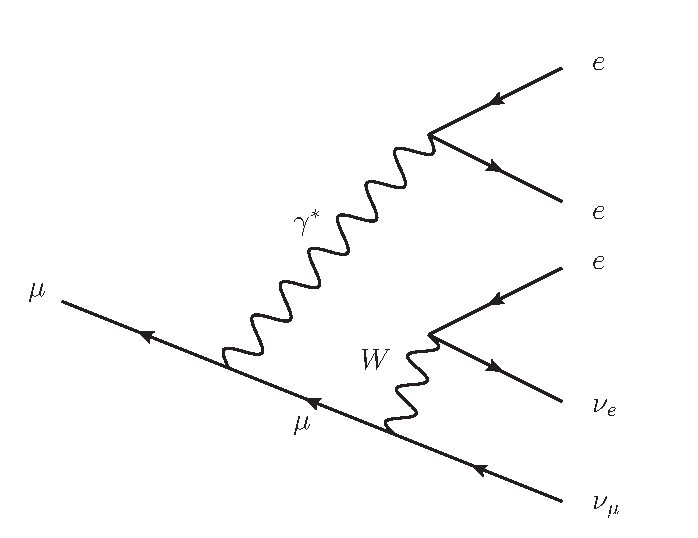
\includegraphics[width = 0.6\textwidth]{Figures/feynman_diagrams/mu_eeenunu_SM.eps}
    \caption[One Feynman diagram for the SM process $\mu^+ \rightarrow e^+ \bar{\nu}_\mu \nu_e e^+ e^-$ with a virtual photon.]{One Feynman diagram for the SM process $\mu^+ \rightarrow e^+ \bar{\nu}_\mu \nu_e e^+ e^-$. Here a virtual photon is emitted and decays to an $e^+ e^-$ pair. Note that the photon can be radiated off of any of the charged particles in the diagram before the $e^+ e^-$ decay. This background process can be suppressed by using momentum conservation with a high energy resolution.}
    \label{fig:mu_eeenunu_SM}
\end{figure}


Another source of background for the experiment is the radiative muon decay

\begin{equation}
    \mu^+ \rightarrow e^+ + \bar{\nu}_\mu + \nu_e + \gamma
\end{equation}

\noindent where the $\gamma$ radiates off of either the muon or electron.
This process comes with a branching ratio of $1.4 \times 10^{-2}$, given a photon energy larger than $10\textrm{MeV}$ \cite{Agashe:2014kda}.
The photon can then convert to an $e^+ e^-$ pair in the detector or target material and mimic the irreducible background above.
Conversions outside of the target can be suppressed if the vertex can be readily identified.
This conversion process will be a much more important source of background for the low mass range of the scalar, as the $e^+ e^-$ pair from the converted photon will be highly collimated for all but the lowest photon energies.
Within the target, this background appears as an accidental background with a regular muon decay.

There are other sources of background present as well.
We have already briefly mentioned Michel decays, which can be identified by the lack of any negatively charged particle tracks, since the experiment uses a $\mu^+$ beam.
Bhabha scattering from the positrons coming from either the muon decay or a contaminated beam, scattering off of the target material to make an $e^+ e^-$ pair appear from a single vertex.
This process has missing energy from the unaccounted electron in the target material and can be removed similarly to the irreducible background.
Finally, there are also pions that may contaminate the beam and decay either to $\pi^+ \rightarrow e^+ e^+ e^- \nu_e$, or $\pi^+ \rightarrow \mu^+ \nu_\mu \gamma$ with the photon converting to an $e^+ e^-$ pair, which have branching ratios $3.2 \times 10^{-9}$ and $2.00 \times 10^{-4}$ relatively \cite{Agashe:2014kda}.
It is expected that the pion contamination is on the order of $10^{-12}$ for the HiMB~\cite{Blondel:2013ia}, and the small decay rates should also suppress these numbers of events to safely negligible rates.

Using \madgraph, we generate $200,000$ events corresponding to the SM background for our signal, $\mu^+ \rightarrow e^+ \bar{\nu}_\mu \nu_e e^+ e^-$.
We use such a high amount to have properly populated bins near the tails of the distribution, where the likelihood that a bin will be populated is small.
To improve the time required to generate the events, we ignore contributions from the Higgs and the $Z$ bosons, as they will not contribute at energies associated with muon decay.
As a cross-check, the total width we obtain from the SM process is $1.239\times 10^{-23}\textrm{GeV}$, yielding a branching ratio of $4.119\times 10^{-5}$, which is within errors of the PDG value of $(3.4 \pm 0.4) \times 10^{-5}$ \cite{Agashe:2014kda}.

\subsection{Signal}
The signal we are interested in is the spectral feature over the irreducible background present in \mueee.
That is, the process we are investigating has the same final state as $\mu^+ \rightarrow e^+ \bar{\nu}_\mu \nu_e e^+ e^-$, but with the electron and one of the positrons reconstructing the mass of the scalar.

We will be using both the scalar model and the dark photon model here.
The signal processes of interest are the decay chains

\begin{align}
    \mu^+ & \rightarrow e^+ + \bar{\nu}_\mu + \nu_e + \phi,~\phi \rightarrow e^+ + e^- \\
    \mu^+ & \rightarrow e^+ + \bar{\nu}_\mu + \nu_e + A',~A' \rightarrow e^+ + e^-
\end{align}

\noindent with the $\phi$ and $A'$ being produced on-shell.
One diagram for the scalar case can be seen in Fig.\ \ref{fig:mu_eeenunu_scalar}.
All of the diagrams generated by \madgraph that are used can be seen in appendix \ref{app:muon_diagrams}.
Note that while we generate events with the scalar radiating off of either the decaying muon or the positron from the muon decay, the emission from the muon dominates, unlike the QED case, due to the stronger coupling to the muon than the positron.

\begin{figure}[h]
    \centering
    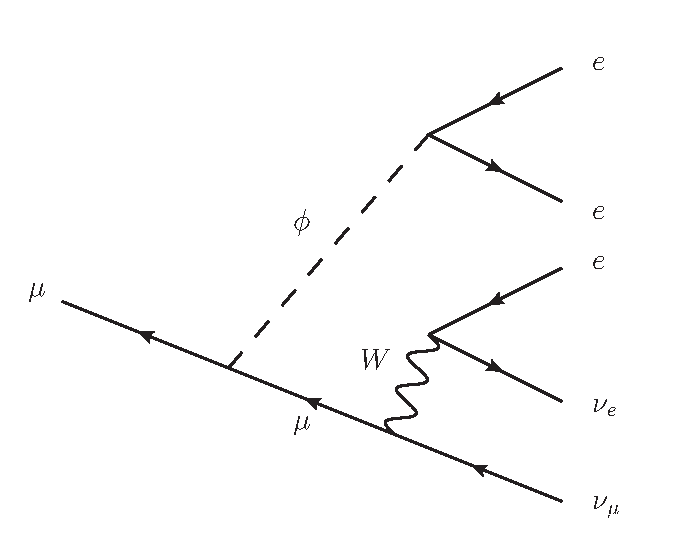
\includegraphics[width=0.6\textwidth]{Figures/feynman_diagrams/mu_eeenunu_scalar}
    \caption[Feynman diagram for the scalar signal in muon decay.]{Feynman diagram for the scalar signal in muon decay. Remember that the scalar is produced on-shell here and can only decay to the $e^+ e^-$ pair.There is a second diagram with the scalar being radiated off of the electron from the $W$ decay instead of off the initial state muon, however the emission off of the muon dominates. Two identical diagrams exist for the dark photon, where the $A'$ replaces the $\phi$.}
    \label{fig:mu_eeenunu_scalar}
\end{figure}

We generate events at $10,000$ events at 200 different mass points, logarithmically spaced from $1.1\textrm{MeV}$, slightly higher than $2m_e$, up to $100\textrm{MeV}$, slightly lower than $m_\mu$.
It's worth briefly noting here that \madgraph does not natively support scanning over a parameter, such as the mass of the mediator.
To get around this, we have written a wrapper around \madgraph in \texttt{Python}, which will directly interface with the \madgraph calls and can automatically run the generator over any parameter scan, with minimal overhead.
For all runs, the coupling to the muon and scalar is set at $g_{\phi\mu} = 0.1$, and will be rescaled later to determine the limiting value.
$10,000$ events were chosen to be generated to reduce the statistical error in each bin, as we will be scaling the number of events up to $\sim 10^{16}$ total events.
This was also a sweet spot where the time taken to generate the events on a modern laptop was on the order of a few hours.
The results of generating these events are twofold:
\begin{itemize}
    \item{The total width of the process is given, which we can use to rescale the events. For example,
        \begin{equation}
            \Gamma(m_\phi \approx 21\textrm{MeV}) = 1.3\times 10^{-11}~\Gamma(\mu^+ \rightarrow \textrm{all}) \left(\frac{g_{\phi\mu}}{10^{-4}}\right)^2\textrm{.}
        \end{equation}
        \madgraph tallies this partial width for us. This will capture the overall behaviour of our signal, corresponding to the total number of raw signal events all placed into one bin.}
    \item{A collection of events with the four-momentum for each particle, and their parents if they are a decay product are output by the program. We can use these to plot the spectrum of the decay products.}
\end{itemize}

Once we have a collection of events, we can bin the results in a relevant parameter and use the spectrum to place limits on the sensitivity of \mueee.
A natural choice here is to plot the histogram of events in the invariant mass of the $e^+ e^-$ pair.
Since the scalar is decaying on-shell and has a narrow width, the invariant mass of its decay products must equal the mass of the parent.
This yields a resonant ``bump'' in the decay spectrum at the mass of the scalar, and the signal spectrum behaves as a delta-function.
In reality, of course, this delta-function will be broadened by {\em e.g.}\ detector resolution.
Since the final state has two positrons, it is not clear which to use when constructing the invariant mass spectrum.
These should be back to back, but only in the rest frame of the scalar, so that there are no obvious selection cuts one can apply on an event-by-event level.
However, for our simple analysis, we construct both available pairs and simply correct by a factor of two.
Note that while we know the true parent particle, we do not make use of this information to better reflect an experimental search for the scalar.

The choice of binning is very important.
If they are too wide, the signal features can be spread across a wide number of background events in the same bin.
On the other hand, we are limited by the detector's tracking and energy resolution.
Through private communication in August 2014 with Dr.~Andre Sch\"oning, the contact person at \mueee, we have been told that the mass resolution is $\sigma_m / m \approx 0.004$.
This holds best for the heavier mediators in the mass range of $10 - 100~\textrm{MeV}$.
Lighter invariant mass pairs, $\sim 1~\textrm{MeV}$, are harder to distinguish, as the decay angle is small and the resolution is limited by multiple scattering.
For now, we simply use the mass resolution at $10~\textrm{MeV}$, for the low mass limit of our generated events, but one must keep in mind that below $10~\textrm{MeV}$ the results will likely be overly optimistic.

With this mass resolution in mind, we bin each of the invariant mass spectra.
After scaling up the total number of events to $10^{15}~(5.5\times 10^{16})$ for \mueee phase I (phase II), scaling the signal events by the branching ratio of the signal, and scaling the background events by the SM branching ratio, we are ready to use the spectrum.
We also rescaled by a factor of $137 / 127.9$ for the running of the $\alpha$ coupling, as \madgraph by default uses $\alpha$ evaluated at the mass of the $Z$.
The scaling by the branching ratios ensures that we have the correct number of expected total signal events, and background events.
An example spectrum with both signal and background is shown in Fig.~\ref{fig:mu_eeenunu_spectrum}.

\begin{figure}[t]
    \centering
    \begin{subfigure}[b]{0.45\textwidth}
        \centering
        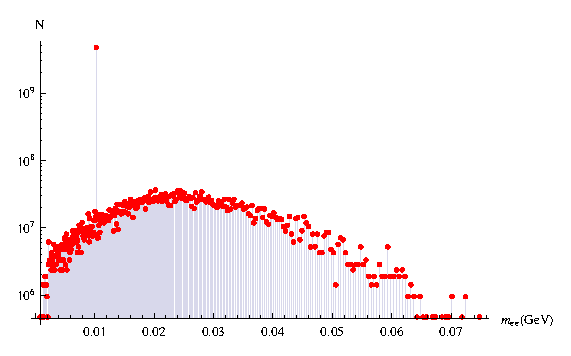
\includegraphics[width=\textwidth]{Figures/spectra/mu_eeenunu_scalar}
        \label{fig:mu_eeenunu_scalar_spectrum}
    \end{subfigure}
    \begin{subfigure}[b]{0.45\textwidth}
        \centering
        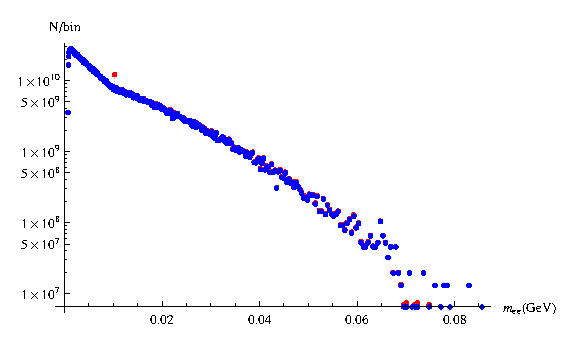
\includegraphics[width=\textwidth]{Figures/spectra/mu_eeenunu_scalar_background}
        \label{fig:mu_eeenunu_scalar_background_spectrum}
    \end{subfigure}
    \caption[Sample invariant mass spectrum from events generated by \madgraph.]{Sample invariant mass spectrum from events generated by \madgraph. Events in red correspond to signal events, and events in blue correspond to background events.
            \textbf{Left}: The signal spectrum. Note the narrow resonance corresponding to the production of the scalar mediator. The smooth variation below the resonance is attributed to the reconstruction of the $e^+e^-$ pair using the positron whose parent is not the $\phi$. To enhance the peak visibility, $g_{\phi\mu} = 0.01$ is used.
            \textbf{Right}: The signal and background spectrum. The resonance is slightly visible above the background, centered at the mass used during generation. Elsewhere on the spectrum the signal is not visible.}
    \label{fig:mu_eeenunu_spectrum}
\end{figure}

Once we have a spectrum, it is easy to find the limiting coupling according to our prescription in section \ref{sec:limit_procedure} and equation \ref{eqn:gphi_limit}.
Instead of analyzing the total number of signal and background events, we can do better by using the spectrum and focusing on the region where the resonance occurs.
This reduces the background within the bin to a much more reasonable level for sensitivity, and also keeps all of the signal, since we are dealing with a very narrow width.
To implement this, we ask for the bin with maximum signal, look up the corresponding background level, and compute $g_{\phi\mu}^\textrm{limit}$ to $3\sigma$.
The resulting sensitivity limits are shown in Fig.\ \ref{fig:mu3e_limits}.

\begin{figure}[h]
    \centering
    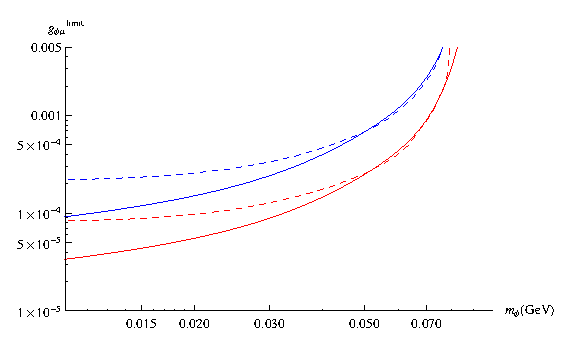
\includegraphics[width=0.5\textwidth]{Figures/limits/mu3e_all}
    \caption[Sensitivity limits on the scalar coupling to muon using $\mu^+$ decay at \mueee.]{Sensitivity limits on the scalar coupling to muon using $\mu^+$ decay at \mueee. Results using our background simulation are shown as solid lines, while results translated using Echenard et.\ al.\ are shown as dashed lines \cite{Echenard:2014lma}. In blue are the phase I limits, and in red are the phase II limits. The dark photon results should have a more robust background and detector simulation than our simple treatment. Our background simulation allows for sensitivity limits lower than $10\textrm{MeV}$, however the resolution of the invariant mass of the $e^+ e^-$ pair is relatively unknown here, so we limit ourselves to $m_\phi > 10~\textrm{MeV}$.} 
    \label{fig:mu3e_limits}
\end{figure}

We also make use of an existing study of the dark photon at the \mueee experiment to obtain limits in a similar fashion.
Echenard et.\ al.\ have done this using a similar method, using \madgraph to generate events and then inserting a proper detector simulation \cite{Echenard:2014lma}.
Their limits extend for a dark photon mass range of $10 - 80~\textrm{MeV}$, as the dark photon is mostly ruled out already below $10~\textrm{MeV}$.
This removes any need for us to do background simulation for this case.
In order to translate their limits from the dark photon case to the scalar case, we must do a simple simulation of the dark photon signal ourselves.
Using the dark photon model developed earlier for \madgraph, we perform the same generation of events as outlined for the scalar.
We set the dark photon kinetic mixing to $\epsilon = 0.1$, and generate signal events over the same 200 mass points.
Equating the number of signal events between the two models for the given limiting $\epsilon$ and an unknown limiting $g_{\phi\mu}$, let us translate the limits, since the number of events detected for sensitivity must be the same.
Doing this, we find the following result:

\begin{equation}
    g_{\phi\mu}^\textrm{limit} = g_{\phi\mu}^\textrm{test} \frac{\epsilon^\textrm{limit}}{\epsilon^\textrm{test}}\sqrt{\frac{\textrm{BR}(\mu^+ \rightarrow e^+ \bar{\nu}_\mu \nu_e A')}{\textrm{BR}(\mu^+ \rightarrow e^+ \bar{\nu}_\mu \nu_e \phi)}}
    \label{eqn:gphi_limit_echenard}
\end{equation}

\noindent In this expression, the branching ratios and $\epsilon^\textrm{limit}$ are all a function of mass, with the branching ratios coming from our simulation and the limiting kinetic mixing from~\cite{Echenard:2014lma}.
The resulting limits can be seen in Fig.~\ref{fig:mu3e_limits}.

Comparing the results of the two methods, the plateauing behaviour towards low mass mediators is more likely correct than our treatment of a fixed mass resolution below $10\textrm{MeV}$.
As expected, our results are more optimistic.
This is likely because we are not taking into account detector efficiencies, which will degrade the signal sensitivity towards the lower masses.
Nonetheless, the agreement everywhere towards the higher mass end suggests that our simulation is robust enough while also being relatively simple in concept.
